% ------------------------------------------------------------------------
% ------------------------------------------------------------------------
% ICMC: Modelo de Trabalho Acadêmico (tese de doutorado, dissertação de
% mestrado e trabalhos monográficos em geral) em conformidade com 
% ABNT NBR 14724:2011: Informação e documentação - Trabalhos acadêmicos -
% Apresentação
% ------------------------------------------------------------------------
% ------------------------------------------------------------------------

% Opções: 
%   Qualificação         = qualificacao 
%   Curso                = doutorado/mestrado
%   Situação do trabalho = pre-defesa/pos-defesa (exceto para qualificação)
% -- opções do pacote babel --
% Idioma padrão = brazil
	%spanish,			% idioma adicional para hifenização
	%english,			% idioma adicional para hifenização
	%brazil				% o último idioma é o principal do documento
\documentclass[mestrado, spanish, english, brazil]{packages/icmc}

% ---
% Pacotes Opcionais
% ---
\usepackage{rotating}           % Usado para rotacionar o texto
\usepackage[all,knot,arc,import,poly]{xy}   % Pacote para desenhos gráficos
% Este pacote pode conflitar com outros pacotes gráficos como o ``pictex''
% Então é necessário usar apenas um dos pacotes conflitantes

\newcommand{\VerbL}{0.52\textwidth}
\newcommand{\LatL}{0.42\textwidth}


% ---
% Informações de dados para CAPA e FOLHA DE ROSTO
% ---
\titulo{Avaliação e dimensionamento de muros executados com resíduos de construção e demolição reciclados e reforçados com geogrelha}
\autor[Neuhaus, L. A.]{Lucas Arendt Neuhaus}
\orientador[Orientador]{Prof. Dr.}{Jefferson Lins da Silva}
%\coorientador{Prof. Dr.}{Fulano de Tal}
\curso{CCMC}
\data{5}{9}{2018} % Data do depósito
% ---


% ---
% RESUMOS
% ---

% Resumo em português
% conter no máximo 500 palavras
\textoresumo{
    O intenso crescimento das cidades traz consigo a preocupação com a exploração abusiva dos recursos naturais não renováveis, e por conta disso a adoção de alternativas sustentáveis tornam-se cada vez mais atrativas e necessárias. A utilização de Resíduos de Construção e Demolição Reciclados (RCD-R) e de solos não convencionais como material de preenchimento para Estruturas de Solo Reforçado (ESR) têm se mostrado uma opção altamente viável. Diante disso, neste trabalho procurou-se analisar e exemplificar a utilização de RCD-R na construção de um muro reforçado com geogrelha.
    
    
    } {Muro, Resíduo de Construção Civil, Geossintético, Geogrelha}

    
    
% ---
% Configurações de aparência do PDF final
% ---
% alterando o aspecto da cor azul
\definecolor{blue}{RGB}{41,5,195}

% informações do PDF
\makeatletter
\hypersetup{
     	pagebackref=true,
		pdftitle={\@title}, 
		pdfauthor={\@author},
    	pdfsubject={\imprimirpreambulo},
	    pdfcreator={LaTeX with abnTeX2/ICMC-USP},
		pdfkeywords={\palavraschave}, 
		colorlinks=true,       		% false: boxed links; true: colored links
    	linkcolor=black,          	% color of internal links
    	citecolor=black,        		% color of links to bibliography
    	filecolor=magenta,      	% color of file links
		urlcolor=black,
		bookmarksdepth=4
}
\makeatother
% --- 

% ----------------------------------------------------------
% ELEMENTOS PRÉ-TEXTUAIS
% ----------------------------------------------------------

% Inserir a ficha catalográfica
% \incluifichacatalografica*{tex/fichaCatalografica.pdf}
 \incluifichacatalografica*{tex/pre-textual/PaginaEmBranco.pdf} % Código Cutter: número atribuído ao sobrenome do autor. Para obtê-lo, consulte a tabela Cutter Sanborn (em http://www.davignon.qc.ca/cutter1.html), procure pelo sobrenome ou forma mais próxima ao sobrenome completo e coloque o número indicado como parâmetro.


% DEDICATÓRIA / AGRADECIMENTO / EPÍGRAFE
% \textodedicatoria*{tex/pre-textual/dedicatoria}
% \textoagradecimentos*{tex/pre-textual/agradecimentos}
% \textoepigrafe*{tex/pre-textual/epigrafe}

% Inclui a lista de figuras
 \incluilistadefiguras

% Inclui a lista de tabelas
 \incluilistadetabelas

% Inclui a lista de quadros
% \incluilistadequadros

% Inclui a lista de algoritmos
% \incluilistadealgoritmos

% Inclui a lista de códigos
% \incluilistadecodigos

% Inclui a lista de siglas e abreviaturas
% \incluilistadesiglas

% Inclui a lista de símbolos
% \incluilistadesimbolos

% ----
% Início do documento
% ----
\begin{document}
% ----------------------------------------------------------
% ELEMENTOS TEXTUAIS
% ----------------------------------------------------------
\textual

\chapter{Resumo do TCC 1}
\label{resumotcc1}
\section{Resumo do relatório final do TCC 1}
A disciplina Trabalho de Conclusão de Curso I foi realizada no Departamento de Estruturas (SET), no segundo semestre de 2017, portanto o tema escolhido era outro, assim como o professor orientador. Alguns imprevistos impossibilitaram a continuação do TCC 1, em seu percurso natural, no primeiro semestre de 2018. A decisão tomada foi a procura de um novo tema, para ser concluído na duração deste semestre.

\section{Progresso}
Até então foi realizado um profundo estudo sobre os assuntos referentes ao tema, contando com a análise das leis que regem o destino dos resíduos da construção civil, como a Resolução CONAMA 307/2002, a tese de Eder Carlos Guedes dos Santos sobre a avaliação experimental de muros executados com RCD-R, entre diversos outros. Foi possível verificar o interesse da comunidade acadêmica brasileira em aprimorar e incentivar o uso de Resíduos de Construção Civil visto a quantidade de estudos disponíveis.

Os materiais disponíveis sobre geossintéticos também são muitos, em especial o Manual Brasileiro de Geossintéticos e o excelente site \textit{www.geoacademy.com.br}.

\section{Dificuldades encontradas}
A principal dificuldade encontrada foi o prazo de realizar todo o projeto em apenas um semestre, mas com certeza não é algo que inviabiliza a execução do mesmo.

\chapter{Introdução}
\label{chapter:introducao}
% Comando simples para exibir comandos Latex no texto
\newcommand{\comando}[1]{\textbf{$\backslash$#1}}

\section{Considerações Gerais}

Testando a inserção de uma nova sigla \sigla{EESC}{Escola de Engenharia de São Carlos}, vamos ver se deu certo.

\sigla{ESR}{Estrutura de Solo Reforçado}

\sigla{RCD}{Resíduo de Construção e Demolição}

\sigla{RCD-R}{Resíduo de Construção e Demolição Reciclado}


\begin{table}[htb]
\IBGEtab{%
  \caption{População dos países da América do Sul} \label{tabela:populacao_america_sul_nova}
}{%
\begin{tabular}{r|p{3cm}|r}        
\toprule
Código  & País            & População   \\ \midrule \midrule
1       & Brasil          & ~~~~~~191.480.630 \\ \midrule 
2       & Argentina       &  39.934.100 \\ \midrule 
3       & Colômbia        &  46.741.100 \\ \midrule 
4       & Paraguai        &   9.694.200 \\ \midrule 
5       & Uruguai         &   3.350.500 \\ \midrule 
6      & Chile           &  16.803.000 \\ \bottomrule
\end{tabular}
}{%
  \fdireta{wikipedia:2011:america_sul}%
  \nota{Esta é uma nota, que diz que os dados são baseados na
  regressão linear.}%
  \nota[Anotações]{Uma anotação adicional, que pode ser seguida de várias
  outras, porém são opcionais.}%
  }
\end{table}

\begin{table}[htb]
\caption{Editores de Texto Livres}
\label{quadro:editores_texto_livres_novo}
\centering
\begin{tabular}{|l|l|r|}        \hline
Editor     & Multiplataforma & Específico para Latex \\ \hline
Kwriter    & Sim             & Não                   \\
Texmaker   & Sim             & Sim                   \\
Kile       & Sim             & Sim                   \\
Geany      & Sim             & Não                   \\ \hline
\end{tabular}
\end{table}

\begin{figure}[htb]
 \caption{Logomarca da USP}
 \label{fig:logomarca_usp_novo}
 \centering
 
\includegraphics[scale=0.3]{usp-logo.pdf}
 \fdireta{usp:logo}
\end{figure}



Este documento explica brevemente como trabalhar com a classe \LaTeX~\textit{icmc} para confeccionar trabalhos acadêmicos seguindo as normas da \sigla{ABNT}{Associação Brasileira de Normas Técnicas} e as \aspas{\textit{Diretrizes para apresentação de dissertações e teses da USP: documento eletrônico e impresso. Parte I (ABNT)}}, publicado pelo \sigla{SIBi}{Sistema Integrado de Bibliotecas} USP. O presente manual também atende as exigências prevista no regimento do Programa de Pós-graduação em \sigla{CCMC}{Ciências da Computação e Matemática Computacional} do \sigla{ICMC}{Instituto de Ciências Matemáticas e de Computação} da \sigla{USP}{Universidade de São Paulo}.


A classe \textit{icmc} foi construída com base na última versão da classe \textit{abntex2} e do pacote \textit{abntex2cite}. Portanto, este documento exemplifica a elaboração de trabalho
acadêmico (tese, dissertação e outros do gênero) produzido conforme a ABNT NBR
14724:2011 \textit{Informação e documentação - Trabalhos acadêmicos - Apresentação}.

Assim, é altamente recomendável que seja consultada a documentação do \textit{abntex2}\footnote{https://code.google.com/p/abntex2/downloads/list}. A classe \textit{abntex2} foi desenvolvida para facilitar a escrita de documentos seguindo as normas da ABNT no ambiente \LaTeX\;\cite{frasson:2005:classe_abnt}.

Todo o trabalho de pesquisa e ajustes da presente classe \LaTeX~\emph{icmc} foram feitos pelo aluno mestrado do Programa de Pós-graduação em Ciência da Computação e Matemática Computacional, Humberto Lidio Antonelli, durante a confecção da sua monografia de qualificação.

O requisito básico para utilização da classe \textit{icmc} é criar um documento desta classe com o comando
\comando{documentclass[@parameters]\{icmc\}} e ter, no diretório de trabalho, o arquivo \emph{icmc.cls} presente. Entretanto, recomenda-se fortemente manter a estrutura de diretório inicial fornecida por este modelo. Além disso, para que o documento esteja em conformidade com as normas exigidas pelo programa de Pós-Graduação, o \textbf{projeto deve ser compilado utilizando \textit{XeLaTeX} ou \textit{LuaLaTeX}}. Esse processo de compilação é necessário para que as fontes externas utilizadas para gerar a capa sejam incluídas.

Os parâmetros possíveis utilizados pelo \comando{documentclass} são:
\begin{description}
\item[qualificacao] Exclusivamente para monografias de qualificação em geral;
\item[mestrado / doutorado] Identifica o curso ao qual o aluno pertence, sendo utilizado apenas uma das duas opcões disponíveis. O valor padrão é \textbf{doutorado};
\item[pre-defesa / pos-defesa] Identifica a situação do documento (exceto para qualificação), sedo necessário apenas uma das duas opções. O valor padrão é \textbf{pos-defesa};
\item[french, spanish, english, brazil] Adiciona o idioma para correta hifenização correta no documento. O último idioma declarado é o principal do documento. O valor padrão é \textbf{brazil}.
\end{description}

\chapter{Objetivos}
\label{chapter:objetivos}
Este trabalho tem como objetivo o estudo da eficiência e viabilidade da utilização de resíduos de construção e demolição reciclado como material de aterro em muros reforçados com geogrelha. 

Essa análise será feita por meio do dimensionamento e orçamento de uma estrutura em situação comum de solicitação, bem como detalhamento da execução do muro e do seu sistema de drenagem, evitando uma solicitação não prevista na estrutura devido ao empuxo do solo saturado.

O projeto pretende analisar também a situação atual da reciclagem de resíduos na cidade de São Carlos, administrada pela Usina de Reciclagem de Resíduos da Construção Civil da PROHAB. 

\chapter{Revisão Bibliográfica}
\label{chapter:revisao-bibliografica}
\section{Muros}

Muros são estruturas realizadas com a finalidade de conter a movimentação do solo em cortes ou aterro de terrenos. São projetados quando a inclinação do talude em relação a horizontal é superior a 70º, e são compostos por reforço, aterro e elementos da face.

Os muros podem ser reforçados externamente ou internamente. Muros reforçados externamente são por exemplo muro de arrimo e muros de gravidade, em que o solo é apenas uma sobrecarga. Muros reforçados internamente, por outro lado, consideram o solo não apenas como material de construção para o muro como também se beneficiam da resistência do solo para compor a estrutura, como é o caso de muros de aterro reforçado com geossintéticos.

A ideia de introduzir uniformemente elementos de reforço no interior do material de aterro de um muro de suporte,  fez com que a concepção tradicional de estruturas de suporte de terras fosse alterada, sendo cada vez mais estudadas soluções atrativas visualmente e que não têm os aspetos de segurança e econômico como únicas preocupações. O primeiro muro de solo reforçado da era moderna foi proposto por Henri Vidal, em 1966, em que apresentou o conceito moderno de reforço de solo \cite{vidal:article}, composto por unidades verticais de face flexíveis e longas tiras metálicas colocadas na posição horizontal, e espaçadas horizontal e verticalmente, num aterro granular. 

As primeiras experiências de geossintéticos em taludes e muros de solo reforçado foram estabelecidas em 1981, com geogrelhas, nos Estados Unidos. “Atualmente, a utilização de inclusões de geossintéticos em taludes e muros de solo reforçado tem crescido acentuadamente, principalmente por representar uma alternativa, em geral, econômica e de fácil execução \cite{elias:article}.”

A Figura \ref{fig:face-muro} é referente a uma obra no interior de São Paulo, um muro que chega a até 12 metros de altura, com comprimento total do reforço de 20 metros.

\begin{figure}[htb]
 \caption{Face de um muro de solo reforçado com geogrelha}
 \label{fig:face-muro}
 \centering
 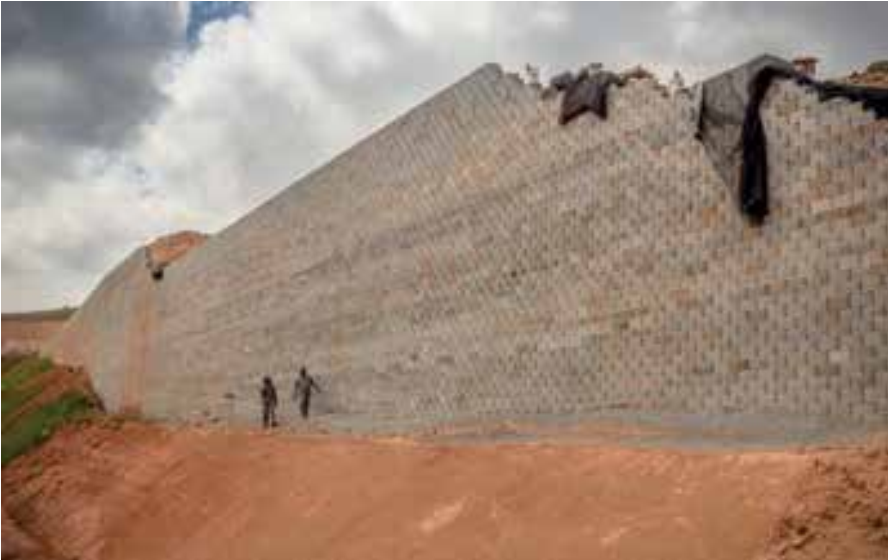
\includegraphics[scale=0.55]{face-muro.PNG}
 \fdireta{lavoie:artigo}
\end{figure}

Um estudo feito em 2001 pelo Departamento de Transporte dos Estados Unidos comparou os custos de execução de algumas soluções de contenção, levando em consideração a altura do muro a ser construído (Figura \ref{fig:custos-muros}. Segundo o estudo, fica clara as vantagens das estruturas de contenção em solos reforçados. Elas são soluções econômicas, capazes de apresentar grande tolerância a recalques de fundações, facilidade construtiva e prazo de execução reduzido. Pode-se acrescentar ainda a vantagem de não exigirem mão de obra especializada.

\begin{figure}[htb]
 \caption{Custos de construção, por área de face, em função da altura do muro, para várias soluções de contenção}
 \label{fig:custos-muros}
 \centering
 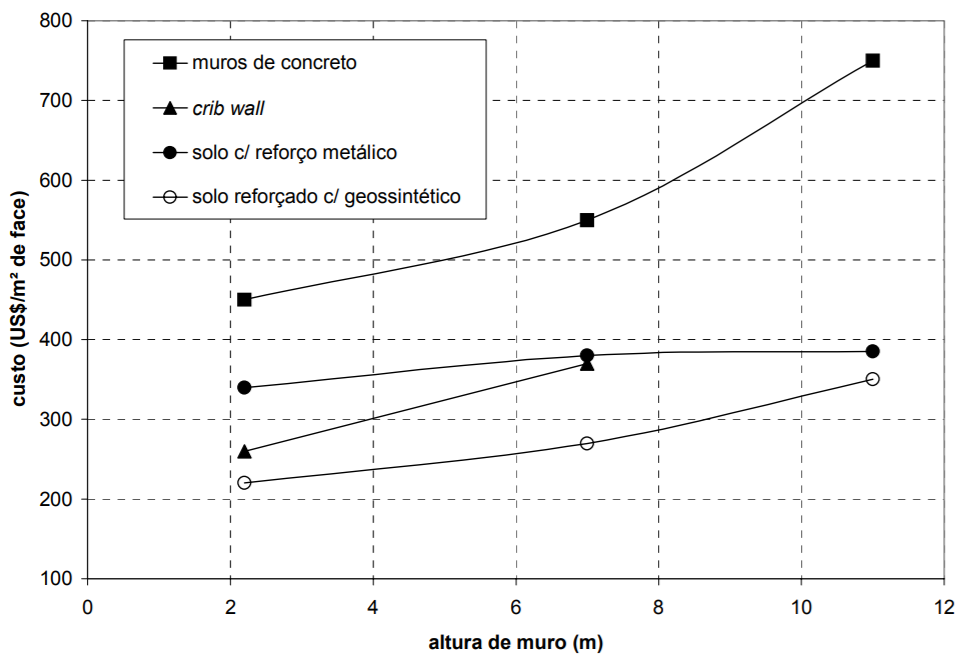
\includegraphics[scale=0.65]{custos-muros.PNG}
 \fdireta{elias:article}
\end{figure}

\section{Resíduos de Construção e Demolição (RCD)}

O ramo da construção civil é um dos mais vastos que compõem a indústria de um país. No Brasil, a construção civil é responsável por gerar mais de 220 mil toneladas de resíduos sólidos urbanos por dia, de acordo com o Panorama de Resíduos Sólidos publicado pela Associação Brasileira de Empresas de Limpeza Pública e Resíduos Especiais(ABRELPE), de 2016. 

Os resíduos sólidos da construção civil são regulamentados pela Política Nacional de Resíduos Sólidos (PNRS) e a Resolução 307/2002 do \sigla{CONAMA}{Conselho Nacional do Meio Ambiente}. A Resolução CONAMA 307 atribui responsabilidade compartilhada sob os resíduos sólidos da construção civil aos geradores, transportadores e gestores municipais.

A definição de RCD, de acordo com o CONAMA, é a seguinte: 

\begin{citacao}
Resíduos de construção civil: são os provenientes de construções, reformas, reparos e demolições de obras de construção civil, e os resultantes da preparação e da escavação de terrenos, tais como: tijolos, blocos cerâmicos, concreto em geral, solos, rochas, metais, resinas, colas, tintas, madeiras e compensados, forros, argamassa, gesso, telhas, pavimento asfáltico, vidros, plásticos, tubulações, fiação elétrica etc., comumente chamados de entulhos de obras, caliça ou metralha \cite{conama:algpseudocode}.
\end{citacao}

A composição dos resíduos sólidos da construção civil é classificada conforme a tabela  \ref{tabela:composicao_residuos_solidos} a seguir, de acordo com as possibilidades de reciclagem.

\begin{table}[htb]
\IBGEtab{%
  \caption{Composição dos resíduos sólidos da construção civil} \label{tabela:composicao_residuos_solidos}
}{%
\begin{tabular}{c|p{6cm}|p{6cm}}        
\toprule
Classe  & Descrição do resíduo & Exemplo   \\ \midrule \midrule
A       
& Materiais que podem ser reciclados ou reutilizados como agregado em obras de infraestrutura, edificações e canteiro de obras.          
& Tijolos, telhas e revestimentos cerâmicos; blocos e tubos de concreto e argamassa. \\ \midrule 
B       
& Materiais que podem ser reciclados e ganhar outras destinações.       
&  Vidro, gesso, madeira, plástico, papelão e outros. \\ \midrule 
C       
& Itens para o qual não existe ou não é viável aplicação econômica para recuperação ou reciclagem.        
&  Estopas, lixas, panos e pincéis desde que não tenham contato com substância que o classifique como D. \\ \midrule 
D       
& Aqueles compostos ou em contato de materiais/substâncias nocivos à saúde.        
&   Solvente e tintas; telhas e materiais de amianto; entulho de reformas em clínicas e instalações industriais que possam estar contaminados. \\ \bottomrule
\end{tabular}
}{%
  \fdireta{conama:algpseudocode}%
  }
\end{table}

A falta de políticas eficientes para a reciclagem e utilização dos resíduos de construção fazem com que a maior parte seja disposto inadequadamente. O RCD disposto inadequadamente polui o solo, deteriora a paisagem urbana, e constitui uma séria ameaça a saúde pública, além de oferecer abrigo para muitas espécies de vetores patogênicos, tais como: ratos, baratas, moscas, vermes, bactérias, fungos e vírus \cite{schneider:master}.

Na cidade de São Carlos, a quantidade de resíduos gerados varia de 250 a 450 ton/dia. Na maioria das vezes, o resíduo de construção civil é disposto em aterros de inertes, reduzindo a vida útil do aterro e degradando o meio ambiente, e em outras situações o resíduo é retirado das obras e disposto clandestinamente em locais como terrenos baldios, margens de rios e de ruas das periferias da Cidade de São Carlos. A Prefeitura compromete recursos, nem sempre mensuráveis, para a remoção ou tratamento desse resíduo.

A PROHAB São Carlos, em atendimento ao Plano Integrado de Gerenciamento de Resíduos de Construção Civil, e através do Programa de Sustentabilidade Ambiental e Social, implantou a Usina de Reciclagem de Resíduos da Construção Civil, inaugurada em dezembro de 2006. O projeto ainda conta com uma fascinante integração social, pois conta com a mão-de-obra de reeducandos da penitenciária Dr. Antônio de Queiroz Filho, do município de Itirapina.

A capacidade de produção da usina é de até 160 ton/dia, a usina não é capaz então de reciclar todo o resíduo gerado pelo município de São Carlos, mas ameniza o problema da disposição irregular. Além do benefício social e ambiental da usina, números mostram  que a produção de agregados com base no resíduo pode gerar economias de mais de 80\% em relação aos preços dos agregados convencionais, e que a partir deste material é possível fabricar componentes com uma economia de até 70\% em relação a similares com matéria-prima não reciclada \cite{prohab:site}.


\section{Reforços de Geossintéticos}

Geossintéticos são produtos industrializados com um ou mais componentes fabricado com polímero sintético ou natural. São especialmente fabricados para serem utilizados em aplicações geotécnicas, hidráulicas, ambientais e de transporte. Geossintéticos (Figura \ref{fig:amostras-geossinteticos}) podem ser responsáveis por diversas funções em uma estrutura, como separação, filtração, drenagem, e, como utilizado no a construção de muros, função de reforço. 

Em estruturas de solo reforçado (ESR) o reforço de geossintético atua de maneira semelhante às armaduras de aço em uma viga de concreto armado, ou seja, é responsável por restringir as deformações e aumentar a resistência do maciço, deve conferir em particular a resistência à tração.

Segundo \cite{manual-geossinteticos}, são inúmeras as vantagens de execução de geossintéticos como elemento de reforço:

\begin{itemize}
    \item Possibilita a construção de taludes e aterros com inclinação acentuadas;
    \item Minimiza o impacto ambiental decorrente das obras de contenção;
    \item Permite a adoção de tipos variados de acabamento da face dos taludes;
    \item Permite a execução de obras em locais de difícil acesso;
    \item Permite o uso de mão de obra não qualificada e equipamentos simples;
    \item Reduz consideravelmente o tempo de construção da obra.
\end{itemize}

\begin{figure}[htb]
 \caption{Amostras de geossintéticos}
 \label{fig:amostras-geossinteticos}
 \centering
 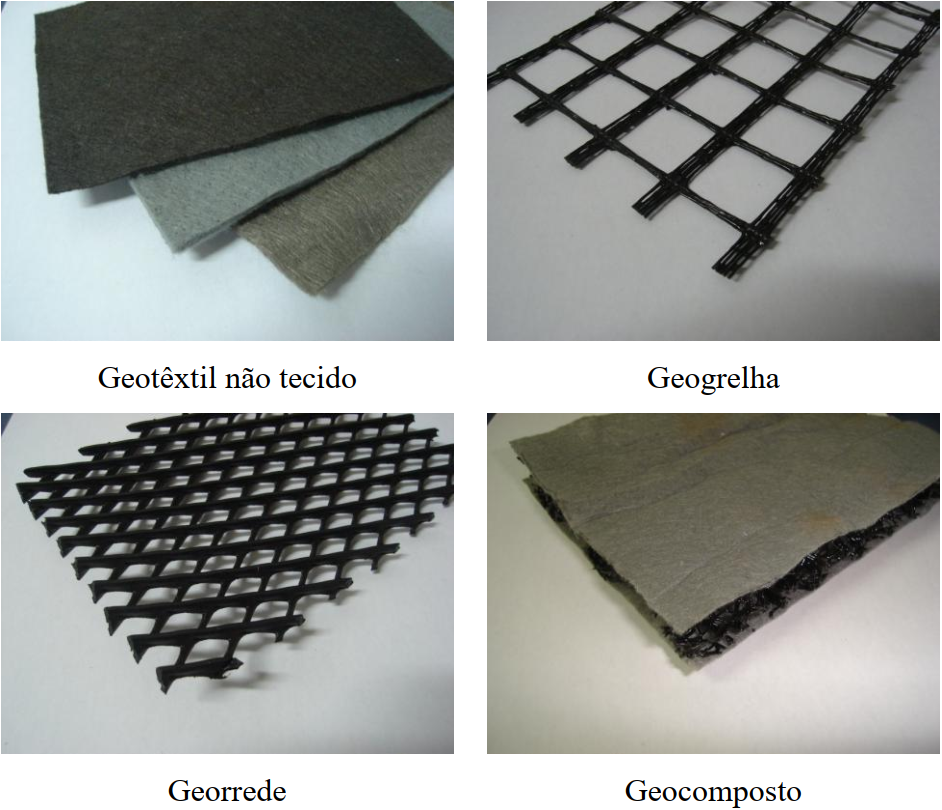
\includegraphics[scale=0.6]{amostras-geossinteticos.PNG}
 \fdireta{santos:2011:master}
\end{figure}




\chapter{Pré-dimensionamento}
\label{chapter:pre-dimensionamento}
O roteiro de dimensionamento para uma estrutura de solo reforçado é muito semelhante ao de uma estrutura não reforçada, com algumas análises diferenciadas devido à presença do reforço e a iteração do reforço com o solo.

Os principais manuais para o dimensionamento de estruturas de solo reforçado são: Federal Highway Administration. American Association of State Highway and Transportation Officials (FHWA, 2002);  \cite{aashto}; e o National Concrete Mansory Association (NCMA, 1997).


São realizadas as seguintes análises para os modos de ruptura:

\begin{itemize}
    \item Estabilidade Externa - Deslizamento, tombamento, capacidade de carga da fundação, e estabilidade global;
    \item Estabilidade Interna - Ruptura do reforço, arrancamento do reforço e conexão do reforço com a face.
\end{itemize}

\section{Estabilidade Externa}

Na análise da estabilidade externa considera-se que a massa de solo reforçado é similar a um muro de gravidade, e deve ser verificada a possibilidade de ocorrer quatro mecanismos clássicos de instabilidade em estruturas de contenção: deslizamento, tombamento, problema de capacidade de carga da fundação e ruptura global (Figura \ref{fig:estabilidade-externa}.

\begin{figure}[htb]
 \caption{Tipos de análise na verificação da estabilidade externa}
 \label{fig:estabilidade-externa}
 \centering
 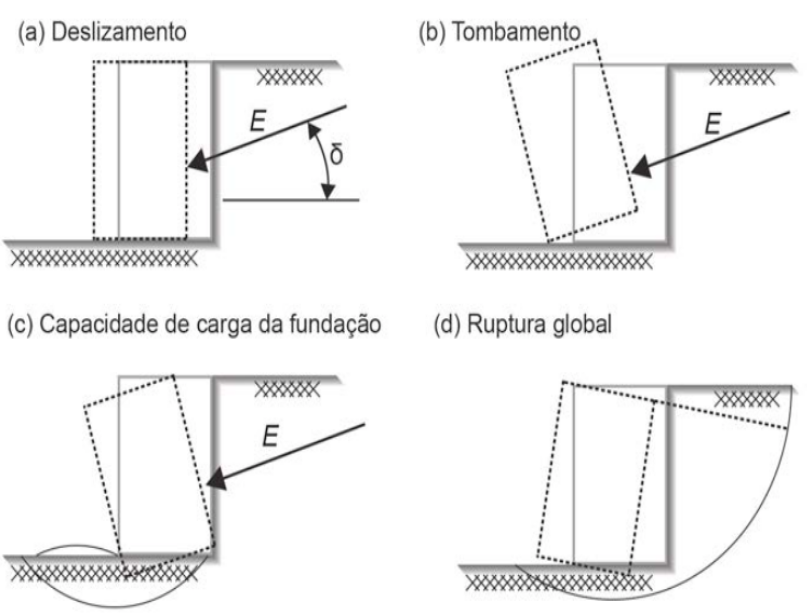
\includegraphics[scale=0.65]{estabilidade-externa.PNG}
 \fdireta{manual-geossinteticos}
\end{figure}

Para a determinação dos empuxos de solo $E$ que a massa de solo não reforçada exerce na massa de reforçada é possível adotar as teorias clássicas de equilíbrio limite. Para os cálculos será utilizada a formulação de Rankine, em que empuxos ativos são admitidos como sendo paralelos à superfície do terreno.

Devem ser consideradas as propriedades de curto e de longo prazos do solo, para verificação das condições durante a construção, durante a vida de serviço da estrutura e também em relação às mudanças que possam ocorrer de pressão neutra. O empuxo passivo atuante no pé do muro ou da estrutura de contenção abaixo do nível do terreno deve ser desprezado, na consideração das forças estabilizantes.

\subsection{Deslizamento}

A verificação da estabilidade ao escorregamento ou deslizamento da estrutura reforçada ao longo da sua base, na interface entre o aterro reforçado e o terreno de apoio, deve ser realizada usando as propriedades do solo reforçado ou do solo de apoio, aquele que for mais desfavorável. O fator de segurança ($FS_d$) utilizado é \textbf{1,5} para obras permanentes.

\begin{equation}
    FS_d = \frac{(\gamma_1 . H + q) . L_d . \tan(\phi)}{E_A} \geq 1,5
\end{equation}

Em que,

$FS_d$: fator de segurança ao deslizamento ao longo da base da estrutura;

$L_d$: comprimento do reforço ou largura da base da estrutura de solo reforçado;

$q$: sobrecarga uniformemente distribuída sobre o terrapleno;

$\gamma_1$: peso específico do solo 1;

$H$: altura da estrutura reforçada;

$\phi$: ângulo de atrito do solo de fundação ou solo do aterro, o que for menor;

$E$: Empuxo ativo calculado por Rankine.


\subsection{Tombamento}

Na verificação da segurança ao tombamento, o fator de segurança é calculado pela razão entre o momento resistente, devido ao peso da estrutura reforçada, e o momento atuante, exercido pelo empuxo de solo $E$. O fator de segurança ($FS_d$) recomendado neste caso é \textbf{2,0}.
 
 \begin{equation}
    FS_t = \frac{(\gamma_1 . H + q) . L_t}{2 . E . y_E} \geq 2,0
 \end{equation}
 
Em que,

$FS_t$: fator de segurança ao tombamento;

$L_t$: largura da estrutura reforçada ou comprimento do reforço;

$\gamma_E$: braço do momento do empuxo ativo, em relação ao pé da estrutura reforçada.
 
 \subsection{Capacidade de Carga da Fundação}
 
 A capacidade de carga máxima $q_{m\Acute{a}x}$ do solo de fundação pode ser avaliada pela equação de \citeonline{terzaghi:article} para uma fundação corrida.
 
 \begin{equation}
    q_{m\Acute{a}x} = c' . N_c + q_S . N_q = 0,5 . \gamma . B' . N_\gamma
 \end{equation}
 
 O fator de segurança para esta verificação é 3,0.
 
 \begin{equation}
 FS_t = \frac{q_{m\Acute{a}x}}{q_r} \geq 3,0
 \end{equation}
 
 Em que,
 
 $q_{m\Acute{a}x}$: capacidade de carga máxima do solo de fundação;
 
 $c'$: coesão do solo de fundação;
 
 $q_s$: sobrecarga ou nível da base da estrutura, caso esteja parcialmente enterrada;
 
 $\gamma$: peso específico do solo de fundação;
 
 $N_c, N_q, N_\gamma$: fatores de capacidade de carga;
 
 $q_r$: fator de capacidade de carga atuante na base do muro ou da estrutura;
 
 $R_v$: resultante das cargas verticais atuantes;
 
 $L$: comprimento do reforço na base do muro ou da estrutura;
 
 $e$: excentricidade da carga resultante $R_v$ em relação a linha central da base de largura $L$.
 
 
\subsection{Estabilidade Global}
 
Na verificação da estabilidade global é realizada a análise da estabilidade do maciço que contém a estrutura de solo reforçado, considerando que esta pode se deslocar como um corpo rígido no interior do maciço. Calcula-se o fator de segurança contra a rotação do maciço considerado, ao longo de uma superfície.

O fator de segurança recomendado é 1,5 e é obtido da seguinte forma:

\begin{equation}
    FS_g = \frac{\sum M_R}{\sum M_A}
\end{equation}

Em que:

$\sum M_R$: somatória dos momentos dos esforços resistentes em relação ao centro de rotação;

$\sum M_A$: somatória dos momentos dos esforços atuantes em relação ao centro de rotação.
 
 
\section{Estabilidade Interna}
 
O método recomendado para as análises da estabilidade interna é o proposto por \citeonline{mitchell:article}. Esse método é de simples aplicação e gera um dimensionamento verificado como adequado na prática.

É importante ressaltar que, por ser uma metodologia de países temperados, inicialmente o método não contempla o uso da coesão efetiva do nos cálculos. Contudo, a consideração desse parâmetro é de simples inserção no método, devendo ser incluído na determinação da força horizontal em cada camada do reforço e na resistência ao arrancamento do mesmo.
 
 Para evitar a ruptura dos reforços, o valor da tensão máxima atuante $T_m\Acute{a}x$ não deverá ser superior ao menor valor esperado para a resistência de projeto do geossintético $T_d$, amparado por um fator de segurança.
 
 A análise da estabilidade interna requer o conhecimento ou a adoção de valores do coeficiente do empuxo horizontal dentro da massa de solo reforçado. Projetistas que não possuem uma grande base de dados de estruturas reforçadas instrumentadas têm adotado o coeficiente de empuxo ativo, constante em toda a altura da estrutura, para a determinação das pressões horizontais.
 
 \subsection{Ruptura do Reforço}
 
 O sistema de reforços deve ser capaz de suportar as pressões transferidas pelo solo, sem romper. A pressão horizontal $\sigma_h$ em qualquer ponto da altura da estrutura pode ser determinada como: 
 
 \begin{equation}
     \sigma_h = k . \sigma_v
 \end{equation}
 Em que: 
 
 $k$: coeficiente de empuxo;
 
 $\sigma_v$: pressão vertical em qualquer profundidade
 
 
 
 \subsection{Arrancamento do Reforço}
 
A resistência ao arrancamento é desenvolvida por dois mecanismos de transferência de tensão, como ilustrado na Figura \ref{fig:transferencia-tensao}: 

\begin{enumerate}
    \item Atrito na superfície plana do reforço;
    \item Resistência passiva na superfície do reforço normal na direção do movimento relativo entre o solo e o reforço.
\end{enumerate}

\begin{figure}[htb]
 \caption{Mecanismos de transferência de tensão entre o solo e a geogrelha}
 \label{fig:transferencia-tensao}
 \centering
 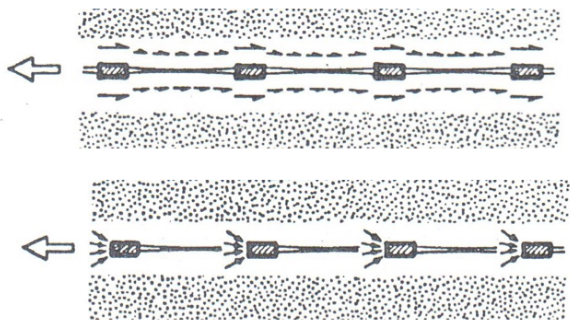
\includegraphics[scale=0.65]{transferencia-tensao.PNG}
 \fdireta{jewell:article}
\end{figure}
 
 
 




\chapter{Cronograma}
\label{chapter:cronograma}
O curto período restante para a entrega final do trabalho traz a necessidade de grande agilidade nas etapas seguintes do trabalho.

\begin{table}[htb]
\IBGEtab{%
  \caption{Cronograma de atividades} \label{tabela:cronograma}
}{%
\begin{tabular}{p{11cm}|p{2cm}|p{2cm}}        
\toprule
Atividade            & Status            & Término   \\ \midrule \midrule

Estudar estruturas de solo reforçado   & Iniciado          & 12/out \\ \midrule 
Analisar a situação atual de geração de RCD-R no Brasil e em São Carlos       & Iniciada        &   15/out \\ \midrule
Dimensionamento dos muros       & Não iniciada        &  20/out \\ \midrule 
Comparativo entre a utilização de solo e RCD como material de aterro       & Não iniciada       &  25/out \\ \bottomrule

\end{tabular}
}{
  }
\end{table}

%\chapter{Exemplos}
%\label{chapter:exemplos}
%% Comando simples para exibir comandos Latex no texto
\newcommand{\comando}[1]{\textbf{$\backslash$#1}}

\section{Considerações Gerais}

Testando a inserção de uma nova sigla \sigla{EESC}{Escola de Engenharia de São Carlos}, vamos ver se deu certo.

\sigla{ESR}{Estrutura de Solo Reforçado}

\sigla{RCD}{Resíduo de Construção e Demolição}

Testando citação \cite{NBR6457:1986}


\begin{table}[htb]
\IBGEtab{%
  \caption{População dos países da América do Sul} \label{tabela:populacao_america_sul_nova}
}{%
\begin{tabular}{r|p{3cm}|r}        
\toprule
Código  & País            & População   \\ \midrule \midrule
1       & Brasil          & ~~~~~~191.480.630 \\ \midrule 
2       & Argentina       &  39.934.100 \\ \midrule 
3       & Colômbia        &  46.741.100 \\ \midrule 
4       & Paraguai        &   9.694.200 \\ \midrule 
5       & Uruguai         &   3.350.500 \\ \midrule 
6      & Chile           &  16.803.000 \\ \bottomrule
\end{tabular}
}{%
  \fdireta{wikipedia:2011:america_sul}%
  \nota{Esta é uma nota, que diz que os dados são baseados na
  regressão linear.}%
  \nota[Anotações]{Uma anotação adicional, que pode ser seguida de várias
  outras, porém são opcionais.}%
  }
\end{table}

\begin{table}[htb]
\caption{Editores de Texto Livres}
\label{quadro:editores_texto_livres_novo}
\centering
\begin{tabular}{|l|l|r|}        \hline
Editor     & Multiplataforma & Específico para Latex \\ \hline
Kwriter    & Sim             & Não                   \\
Texmaker   & Sim             & Sim                   \\
Kile       & Sim             & Sim                   \\
Geany      & Sim             & Não                   \\ \hline
\end{tabular}
\end{table}

\begin{figure}[htb]
 \caption{Logomarca da USP}
 \label{fig:logomarca_usp_novo}
 \centering
 
\includegraphics[scale=0.3]{usp-logo.pdf}
 \fdireta{usp:logo}
\end{figure}



Este documento explica brevemente como trabalhar com a classe \LaTeX~\textit{icmc} para confeccionar trabalhos acadêmicos seguindo as normas da \sigla{ABNT}{Associação Brasileira de Normas Técnicas} e as \aspas{\textit{Diretrizes para apresentação de dissertações e teses da USP: documento eletrônico e impresso. Parte I (ABNT)}}, publicado pelo \sigla{SIBi}{Sistema Integrado de Bibliotecas} USP. O presente manual também atende as exigências prevista no regimento do Programa de Pós-graduação em \sigla{CCMC}{Ciências da Computação e Matemática Computacional} do \sigla{ICMC}{Instituto de Ciências Matemáticas e de Computação} da \sigla{USP}{Universidade de São Paulo}.


A classe \textit{icmc} foi construída com base na última versão da classe \textit{abntex2} e do pacote \textit{abntex2cite}. Portanto, este documento exemplifica a elaboração de trabalho
acadêmico (tese, dissertação e outros do gênero) produzido conforme a ABNT NBR
14724:2011 \textit{Informação e documentação - Trabalhos acadêmicos - Apresentação}.

Assim, é altamente recomendável que seja consultada a documentação do \textit{abntex2}\footnote{https://code.google.com/p/abntex2/downloads/list}. A classe \textit{abntex2} foi desenvolvida para facilitar a escrita de documentos seguindo as normas da ABNT no ambiente \LaTeX\;\cite{frasson:2005:classe_abnt}.

Todo o trabalho de pesquisa e ajustes da presente classe \LaTeX~\emph{icmc} foram feitos pelo aluno mestrado do Programa de Pós-graduação em Ciência da Computação e Matemática Computacional, Humberto Lidio Antonelli, durante a confecção da sua monografia de qualificação.

O requisito básico para utilização da classe \textit{icmc} é criar um documento desta classe com o comando
\comando{documentclass[@parameters]\{icmc\}} e ter, no diretório de trabalho, o arquivo \emph{icmc.cls} presente. Entretanto, recomenda-se fortemente manter a estrutura de diretório inicial fornecida por este modelo. Além disso, para que o documento esteja em conformidade com as normas exigidas pelo programa de Pós-Graduação, o \textbf{projeto deve ser compilado utilizando \textit{XeLaTeX} ou \textit{LuaLaTeX}}. Esse processo de compilação é necessário para que as fontes externas utilizadas para gerar a capa sejam incluídas.

Os parâmetros possíveis utilizados pelo \comando{documentclass} são:
\begin{description}
\item[qualificacao] Exclusivamente para monografias de qualificação em geral;
\item[mestrado / doutorado] Identifica o curso ao qual o aluno pertence, sendo utilizado apenas uma das duas opcões disponíveis. O valor padrão é \textbf{doutorado};
\item[pre-defesa / pos-defesa] Identifica a situação do documento (exceto para qualificação), sedo necessário apenas uma das duas opções. O valor padrão é \textbf{pos-defesa};
\item[french, spanish, english, brazil] Adiciona o idioma para correta hifenização correta no documento. O último idioma declarado é o principal do documento. O valor padrão é \textbf{brazil}.
\end{description}


% ---
% Finaliza a parte no bookmark do PDF, para que se inicie o bookmark na raiz
% ---
\bookmarksetup{startatroot}% 
% ---

% ----------------------------------------------------------
% ELEMENTOS PÓS-TEXTUAIS
% ----------------------------------------------------------
\postextual

% ----------------------------------------------------------
% Referências bibliográficas
% ----------------------------------------------------------
\bibliography{references}

% ----------------------------------------------------------
% Apêndices
% ----------------------------------------------------------

% ---
% Inicia os apêndices
% ---
\begin{comment}


\begin{apendicesenv}

    \chapter{Documento básico usando a classe \textit{icmc}}
    \label{chapter:documento-basico}
    \definecolor{gray}{rgb}{0.4,0.4,0.4}
\definecolor{darkblue}{rgb}{0.0,0.0,0.6}
\definecolor{cyan}{rgb}{0.0,0.6,0.6}
\definecolor{maroon}{rgb}{0.5,0,0}
\definecolor{darkgreen}{rgb}{0,0.5,0}


\lstdefinelanguage{myLatex}
{
    keywords={\titulo},
    alsoletter={-},
    sensitive=false,
    morecomment=[l]{\%},
    morecomment=[s]{/*}{*/},
    morestring=[b]",
    morestring=[b]',
    keywordstyle=\bfseries\color{blue},
    commentstyle=\itshape\color{darkgreen},
    morekeywords={documentclass, titulo, autor, data, orientador, coorientador, curso, textoresumo, incluifichacatalografica, textodedicatoria*, textoagradecimentos*, textoepigrafe*, incluilistadefiguras, incluilistadetabelas, incluilistadequadros, incluilistadealgoritmos, incluilistadecodigos, incluilistadesiglas, incluilistadesimbolos, textual, chapter, postextual, begin, bibliography, end}, 
alsoletter={*, \{, \}, \[, \]},
 morekeywords=[2]{\{, \}, \[, \]},
 keywordstyle=[2]\bfseries\color{blue},
 moredelim=[s][\color{maroon}]{\{}{\}},
    moredelim=[s][\itshape\color{maroon}]{\[}{\]},
}

%\lstdefinelanguage{TeX}
%{
%moredelim=*[s][\color{maroon}]{\{}{\}}
%otherkeywords={\{, \}, \[, \], \\}
%  morestring=[b]",
%  moredelim=[s][\bfseries\color{maroon}]{<}{\ },
%  moredelim=[s][\bfseries\color{maroon}]{</}{>},
%  moredelim=[l][\bfseries\color{maroon}]{/>},
%  moredelim=[l][\bfseries\color{maroon}]{>},
%  commentstyle=\color{darkgreen},
%  stringstyle=\color{blue},
%  identifierstyle=\color{red},
%  keywordstyle=\bfseries\color{maroon}
%moredelim=[l][\bfseries\color{maroon}]{>},
%commentstyle=\color{darkgreen},
%  stringstyle=\color{blue},
%  identifierstyle=\color{red}, moredelim=[l][\bfseries\color{maroon}]{\{},
%  keywordstyle=\bfseries\color{maroon}
%}

%\lstset{language={[LaTeX]TeX},
%texcsstyle=*\bfseries\color{blue},
%keywordstyle=\bfseries\color{blue},
%commentstyle=\color{darkgreen},
%morecomment=[s][\color{red}]{\{}{\}},
%otherkeywords={$, \{, \}, \[, \]}
%}

%\begin{codigo}[caption={Exemplo de um documento básico}, label={codigo:documento-basico}, language={[LaTeX]TeX},  breaklines=true,morekeywords={titulo, autor, data, orientador, coorientador, curso, textoresumo, incluifichacatalografica, textodedicatoria*, textoagradecimentos*, textoepigrafe*, incluilistadefiguras, incluilistadetabelas, incluilistadequadros, incluilistadealgoritmos, incluilistadecodigos, incluilistadesiglas, incluilistadesimbolos, {\backslash}textual, chapter, postextual}, alsoletter={{\backslash},*},morecomment=[s][\color{red}]{\{}{\}}]
\begin{codigo}[caption={Exemplo de um documento básico}, label={codigo:documento-basico}, language={myLatex},  breaklines=true]
% Documento utilizando a classe icmc
% Opções: 
%   Qualificação         = qualificacao 
%   Curso                = doutorado/mestrado
%   Situação do trabalho = pre-defesa/pos-defesa (exceto para qualificação)
% -- opções do pacote babel --
% Idioma padrão = brazil
	%spanish,			% idioma adicional para hifenização
	%english,			% idioma adicional para hifenização
	%brazil				% o último idioma é o principal do documento
\ documentclass[doutorado, spanish, english, brazil]{packages/icmc}

% Título do trabalho
\titulo{Título da Monografia}

% Nome do autor
\autor[Abreviação]{Nome completo do autor}

% Data do depósito
\data{18}{12}{2012}

% Nome do Orientador
\orientador[Orientador]{Titulação do orientador}{Nome completo do Orientador}

% Nome do Coorientador (caso não exista basta remover)
\coorientador[Coorientador]{Titulação do coorientador}{Nome completo do Coorientador}
% Se coorientadora troque Coorientador: por Coorientadora dentro do colchetes

% Sigla do programa de Pós-graduação (CCMC, MAT, PIPGES, PROFMAT, MECAI)
\curso{CCMC}
% O valor entre colchetes é opcional para este programa

% Resumo
\textoresumo[Idioma]{
Texto do resumo do trabalho.
}{Lista de palavras-chave separada por virgulas}

% ----------------------------------------------------------
% ELEMENTOS PRÉ-TEXTUAIS
% ----------------------------------------------------------

% Inserir a ficha catalográfica
\incluifichacatalografica{634} % Código Cutter: número atribuído ao sobrenome do autor (disponível em http://www.davignon.qc.ca/cutter1.html).

% Incluí o texto da Dedicatória
\textodedicatoria*{tex/pre-textual/dedicatoria}

% Incluí o texto dos Agradecimentos
\textoagradecimentos*{tex/pre-textual/agradecimentos}

% Incluí o texto da Epígrafe
\textoepigrafe*{tex/pre-textual/epigrafe}

% Inclui a lista de figuras
\incluilistadefiguras

% Inclui a lista de tabelas
\incluilistadetabelas

% Inclui a lista de quadros
\incluilistadequadros

% Inclui a lista de algoritmos
\incluilistadealgoritmos

% Inclui a lista de códigos
\incluilistadecodigos

% Inclui a lista de siglas e abreviaturas
\incluilistadesiglas

% Inclui a lista de símbolos
\incluilistadesimbolos

% Início do documento
\begin{document}

% ----------------------------------------------------------
% ELEMENTOS TEXTUAIS
% ----------------------------------------------------------
\textual

\chapter{Introdução}

Capítulo de Introdução

\chapter{Desenvolvimento}

Capítulo de Desenvolvimento

\chapter{Conclusão}

Capítulo de conclusão

% ----------------------------------------------------------
% ELEMENTOS PÓS-TEXTUAIS
% ----------------------------------------------------------
\postextual

% Nome do arquivo com as referências bibliográficas
\bibliography{referencias}

\end{document}

\end{codigo}

\end{apendicesenv}
% ---


% ----------------------------------------------------------
% Anexos
% ----------------------------------------------------------

% ---
% Inicia os anexos
% ---
\begin{anexosenv}

    \chapter{Páginas interessantes na Internet} 
    \label{chapter:paginas-interessantes}
    \begin{description}
 \item[\url{http://www.tex-br.org}] Página em português com diversos tutoriais e referências interessantes sobre \LaTeX;
 \item[\url{http://en.wikibooks.org/wiki/LaTeX}] Livro em formato \textit{wiki} gratuito sobre \LaTeX;
 \item[\url{http://tobi.oetiker.ch/lshort/lshort.pdf}] Ótimo tutorial sobre \LaTeX (possui versão em português \url{http://alfarrabio.di.uminho.pt/~albie/lshort/ptlshort.pdf}, mas a versão em inglês é a mais atual);
 \item[\url{http://code.google.com/p/abntex2/}] Página do abnTeX2, grupo que desenvolve os pacotes e classes em \LaTeX para as normas da ABNT, nos quais a classe \textit{icmc} foi baseada;
\item[\url{http://www.more.ufsc.br}] Página do Mecanismo On-line para Referências  (MORE) desenvolvido pela UFSC;
\item[\url{http://detexify.kirelabs.org/classify.html}] Página para recuperar o código de símbolos em \LaTeX a partir do desenho fornecido pelo usuário.
 \end{description}

\end{anexosenv}
% ---


\end{comment}
\end{document}